\documentclass{article}

\usepackage[utf8]{inputenc}
\usepackage{amsmath}
\usepackage{amssymb}
\usepackage{amsfonts}
\usepackage{setspace}
\usepackage{algorithm2e}
\usepackage{graphicx}

\usepackage[top=0.75in, bottom=0.75in, left=1in, right=1.25in]{geometry}

\title{CSCI / MATH 2072U - Assignment 4}
\author{Syed Arham Naqvi \\ \small{100590852}}
\date{\today}

\begin{document}

\maketitle


\subsubsection*{QUESTION 1}

\vspace{10pt}

\begin{enumerate}

    \item[(b)]  We can visualize the convergence for the newton method applied to nonlinear system with 2 equations and 2 unknowns.
            
                \begin{figure}[h]
                \centering
                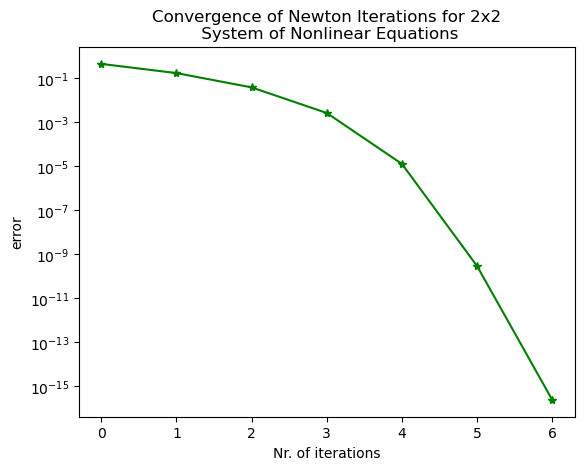
\includegraphics[width=4in]{./Quest1b.png}
                \caption{Nonlinear system convergence.}
                \label{fig:image1}
                \end{figure}
    
    \item[(c)]  The solution for part b:
                \begin{align*}
                    \text{solution vector } \mathbf{x} &= [0.86406221, 0.34086698]^{T}\\
                                                 x_{1} &= 0.86406221\\
                                                 x_{2} &= 0.34086698\\
                \end{align*}
                Based on visual inspection of the plot above, the convergence seems quadtratic just like that of single nonlinear equations.
                Further analysis of the residulas and errors per iteration for the nonlinear system also indicates that the convergence is
                roughly quadratic. However, when compared with the convergence rate of a single nonlinear equation we can see that the rates
                are not exactly the same. With a good initial guess, a single nonlinear equation has a convergence rate that is much closer
                to quadratic then that of the system in this question. This can be observed by squaring the residual for each iteration
                and seeing how close the answer is to the true residual for the next iteration. In this case the square of each residual is
                close to the next residual for the first few iterations until the 4th iteration from which point the next residual is roughly
                equal to the previous raised to the power of 1.5. 


\end{enumerate}
\newpage

\subsubsection*{QUESTION 2}

\vspace{10pt}

\begin{enumerate}

    \item[(a)]  Interpolating polynomial:

                \begin{equation}
                    P_{2}(x) = 2 + 0.45741x - 0.26838x^{2}
                \end{equation}

                \vspace{10pt}

    \item[(b)]  Here we see how well our Polynomial Interpolant in (1) approximates the orginial function:\\ $f(x)=e^{x/2}+\cos(x)$.

                \begin{figure}[h]
                \centering
                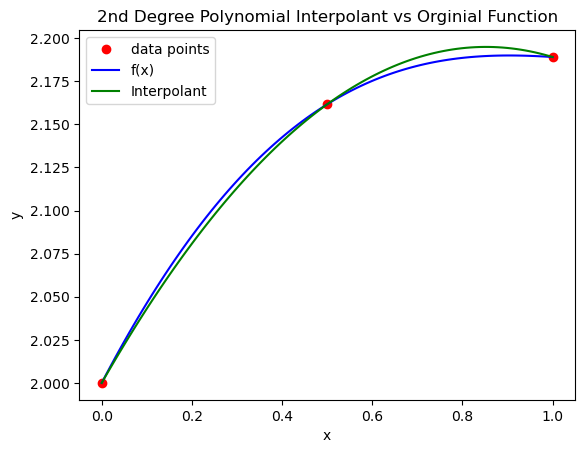
\includegraphics[width=4in]{./Quest2b.png}
                \caption{Accuracy of Polynomial Interpolant}
                \label{fig:image2}
                \end{figure}
            
                \vspace{10pt}

    \item[(c)]  Upper bound for interpolation error on the interval $x\in(0,1)$:
                \begin{align*}
                    |E(x)| = |P_{2}(x)-f(x)| &\leq \underset{ \text{x} \subset \text{I}}{\max} \frac{|f^{(n+1)}(x)|}{(n+1)!}\prod_{k=0}^{n}|x-x_{k}|\\
                                             &\leq \underset{ \text{x} \subset \text{I}}{\max} \frac{|f^{(3)}(x)|}{3!}|x-x_{0}||x-x_{1}||x-x_{1}|\\
                                             &\leq \underset{ \text{x} \subset \text{I}}{\max} \frac{|(\frac{1}{8})e^{x/2}+\sin{x}|}{3!}|x||x-0.5||x-1.0|\\
                                             &\leq \frac{|(\frac{1}{8})e^{(1)/2}+\sin{(1)}|}{3!}|(1)||(0)-0.5||(0)-1.0|\\
                                             &\leq \frac{1.048}{3!}(0.5)\\
                                             &= 0.0873333... \\
                \end{align*}
                $\therefore$ upper bound of interpolation error $= 0.087\overline{3}$
                \vspace{10pt}
    
    \newpage

    \item[(d)]  After computing up to the $100^{th}$ derivative of $f(x)$, evaluating each derivative at $10,000$ evenly spaced
                points in $[0,1]$ and then returning the maximum absolute value of the evaluations, I found that the higher derivatives for
                $f(x)=e^{x/2}+\sin{(x)}$ seem to oscillate between roughly $0.85$ and $1.0$. However, the denominator $(n+1)!$ 
                continues to grow rapidly as the order of interpolation is increased. In addition, because the interval in question is $[0,1]$,
                this means that $\forall x \in [0,1]$ and $k \in [0,1,..,n]$, $|x-x_{k}|\leq 1$ meaning that increasing the order of
                interpolation will only decrease the upper bound of error which must also decrease the interpolation error.

                This finding makes sense since because the maximal value of $|f^{(k)}(x)|$ on the interval $[0,1]$ for $k>0$ shows that the
                higher derivatives of $f(x)$ are small this means that $f(x)$ is a smooth function and so is well-approximated by polynomials.
                Thus, a higher order of interpolation will decrease the interpolation error because the resutling interpolants will be
                polynomials that are not only good apptoxiations of $f(x)$ but will also be equal to $f(x)$ for more points $x_{i} \in [0,1]$. 
                
                \begin{figure}[h]
                    \centering
                    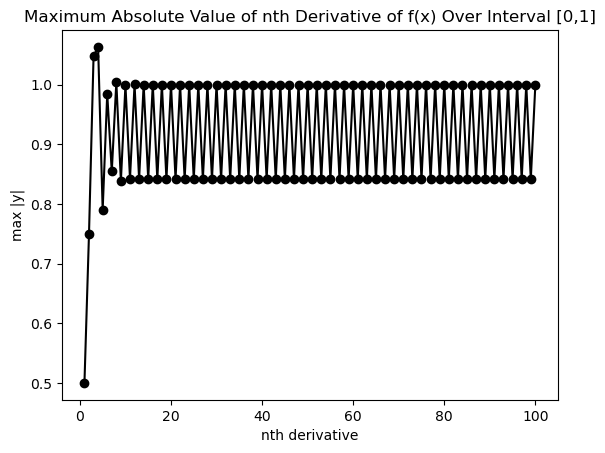
\includegraphics[width=4in]{./Quest2d.png}
                    \caption{Analysis of the nth Derivative of $f(x)=e^{x/2}+\cos(x)$ for $x \in [0,1]$}
                    \label{fig:image3}
                \end{figure}

\end{enumerate}


\subsubsection*{QUESTION 3}

\vspace{10pt}

\begin{enumerate}

    \item[(a)]  What follows is a pseudocode algorithm for constructing matrix M which is the coefficient matrix for
                the linear system used to determine the interpolant $\mathit{\prod_{n}}(x)$ in terms of the Newton
                poylnomial basis. $\bf{M}$ uses mathematical matrix indexing beginning at $1$ and $\bf{x}$ uses $0$-based python indexing.

                \begin{algorithm}[H]
                    \LinesNumbered
                    
                    \KwIn{$(\bf{n}\in\mathbb{N})$ and vector $\bf{x}~s.t~(x\in\mathbb{R}^{(n+1)\times1})$}
                        
                        $M \leftarrow \overline{0}_{(n+1)\times(n+1)}$\\
                        
                        \For{$(i = 1:n+1)$}{
                            
                            $M_{i,1} \leftarrow 1$\\
                            
                            \For{$(j = 2:i)$}{
                                $M_{i,j} \leftarrow M_{i,j-1} \times (x_{i-1}-x_{j-2})$\\
                            }
                        }
                    \KwOut{matrix $\bf{M}~s.t~(M\in\mathbb{R}^{(n+1)\times(n+1)})$}
                \end{algorithm}
                \newpage

    \item[(d)]  The algorithm for part (a) requries the computation of $2$ flops on line $5$.
                This translates to the following computational complexity calculations using flop summations:

                \begin{align*}
                    \text{Computational Complexity} &= \sum_{i=1}^{n+1} \left(\sum_{j=2}^{i}2 \right)\\
                                                    &= \sum_{i=1}^{n+1} \left(2\sum_{k=1}^{i-1}1 \right)\\
                                                    &= 2\sum_{i=1}^{n+1} (i-1)\\
                                                    &= 2\left(\sum_{i=1}^{n+1}i-\sum_{i=1}^{n+1}1 \right)\\
                                                    &= 2\left( \frac{(n+1)((n+1)-1)}{2}-(n+1) \right)\\
                                                    &= (n+1)(n)-2(n+1)\\
                                                    &= n^{2}+n-2n-2\\
                                                    &= n^{2}-n-2\\
                                                    &= \mathcal{O}(n^{2})\\                                     
                \end{align*}
    
    \item[(g)]  What follows is a plot showing the interpolation of a set of data points using the Newton Polynomial Basis:
                \begin{figure}[h]
                    \centering
                    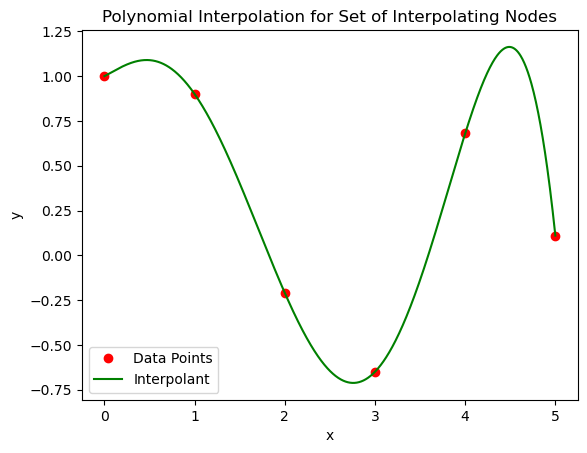
\includegraphics[width=4in]{./Quest3e.png}
                    \caption{Interpolatino using the Newton Polynomial Basis.}
                    \label{fig:image4}
                \end{figure}

\end{enumerate}

\end{document}